%% LyX 2.2.3 created this file.  For more info, see http://www.lyx.org/.
%% Do not edit unless you really know what you are doing.
\documentclass[english]{article}
\usepackage[T1]{fontenc}
\usepackage[latin9]{inputenc}
\usepackage{geometry}
\geometry{verbose,tmargin=2cm,bmargin=2cm,lmargin=2.5cm,rmargin=2.5cm}
\usepackage{float}
\usepackage{graphicx}
\usepackage{setspace}

\makeatletter

%%%%%%%%%%%%%%%%%%%%%%%%%%%%%% LyX specific LaTeX commands.
%% A simple dot to overcome graphicx limitations
\newcommand{\lyxdot}{.}


\makeatother

\usepackage{babel}
\begin{document}
\begin{singlespace}

\title{Project 4: Zombies Outbreak}
\end{singlespace}
\begin{singlespace}

\author{Chenxi Huang, Siyang Jing and Yingqiao Zhou}
\end{singlespace}
\begin{singlespace}

\date{November 27, 2017}
\end{singlespace}

\maketitle
\begin{singlespace}
\noindent \textbf{\Large{}Introduction}{\Large \par}
\end{singlespace}

This report introduces four zombies outbreak models, each of which
is a system of first-order, nonlinear differential equations. We will
use the Heun method to give numerical approximations of these models
and analyze the behaviors of different classes in each model. Specifically,
with one given initial condition of a specific class in a model, we
will evaluate how the changes of initial conditions of other classes
and the changes of parameters influence the decaying rate of that
class. 

\begin{spacing}{1.8}
\noindent \textbf{\Large{}Statement of Problem}{\Large \par}
\end{spacing}

\begin{doublespace}
The four zombie outbreak: Basic model, Latent infection model, Quarantine
model and Treatment model is given as follows. 
\end{doublespace}
\begin{singlespace}
\begin{center}
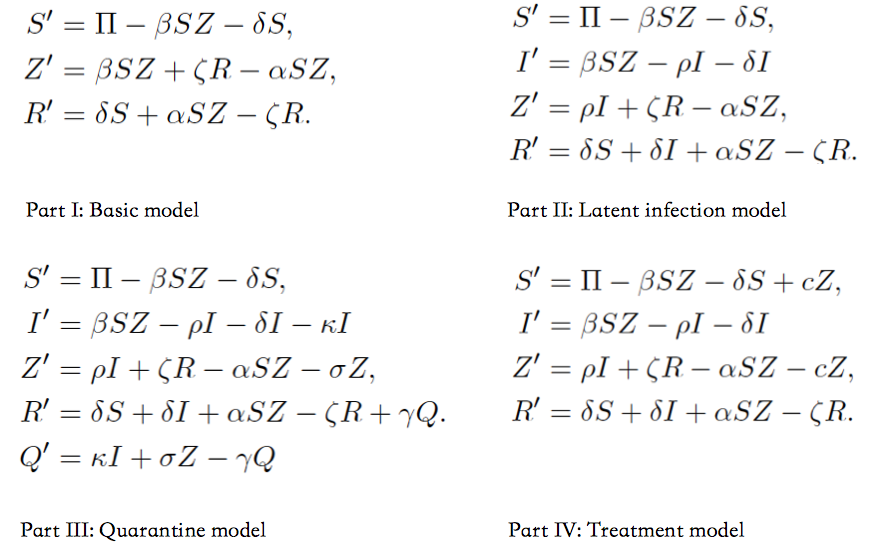
\includegraphics[bb=0bp 0bp 877bp 560bp,clip,scale=0.35]{Figures/model}
\par\end{center}
\end{singlespace}

For all the models above, $S$, $Z$ and $R$ denote the susceptible,
zombie and removed class respectively; I in Part II denote the infected
class and Q in Part III denote the quarantine class; $\Pi,\beta$
and $\delta$ represent the rate of birth, transmission from $Q$
and non-zombie related death rate respectively. $\alpha,\zeta$and
$\rho$represent the rate of zombies defeated, the rate of resurrection
from $R$ to $Z$ and the rate of transmission from $I$ to $Z$.
$\kappa,\sigma$and $\gamma$represent the rates of entering at $Q$
from $I$ , from $Z$ and the rate of I being killed. $c$ represents
the rate of zombies being cured. In this project, $\alpha=\rho=0.005,$
$\beta=0.0095,$ $\zeta=0.0001,$ $\Pi=\delta=0.0001$ and $S(0)=S_{0}=3\times10^{8}.$ 

We need to evaluate under which initial condition $(Z_{0},R_{0})$
would human kind $(S)$ survive in Part I, the effect of the latent
infection $(I)$ to the model in Part II, the effect of quarantine
$(Q)$ to the model in Part III and at which rate$(c)$to treat zombies
so that human kind$(S)$ could survive in Part IV.

\begin{spacing}{1.8}
\noindent \textbf{\Large{}Numerical Method}{\Large \par}
\end{spacing}

To solve for the four models, we will use Heun's method given by the
following formula:
\begin{spacing}{0.3}
\begin{center}
{\footnotesize{}
\begin{equation}
u_{n+1}=u_{n}+\frac{h}{2}[f_{n}+f(t_{n+1},u_{n}+hf_{n})]
\end{equation}
}
\par\end{center}{\footnotesize \par}
\end{spacing}

\begin{doublespace}
Heun's method is an explicit method, which demands less computational
cost than implicit method. An explicit method could be evaluated directly
in terms of known quantities at the previous time step, whereas an
implicit method generally requires a matrix or iterative solution
to compute the new quantities since unknowns are at the both sides
of an equation. Besides, the Heun's method is a method of order 2,
and thereby gives more accurate approximations than first-order methods.
The estimate of truncation error $\tau_{n}$ is derived as follows. 

{\footnotesize{}$\tau_{n}=\frac{u(t_{n+1})-u(t_{n})}{h}-\frac{1}{2}(f_{n}+f(t_{n+1},u(t_{n})+hu'(t_{n})))$}{\footnotesize \par}

{\footnotesize{}$=u'(t_{n})+\frac{h}{2!}u^{(2)}(t_{n})+\mathcal{O}(h^{2})-\frac{1}{2}\left[u'(t_{n})+u'(t_{n})+hf'(t_{n},u_{n})+\mathcal{O}(h^{2})\right]$}{\footnotesize \par}

{\footnotesize{}$=u'(t_{n})+\frac{h}{2}u^{(2)}(t_{n})+\mathcal{O}(h^{2})-\frac{1}{2}(2\cdot u'(t_{n})+hu^{(2)}(t_{n})+\mathcal{O}(h^{2}))=\mathcal{O}(h^{2})$}{\footnotesize \par}
\end{doublespace}

\begin{spacing}{1.8}
\noindent \textbf{\Large{}Analysis}{\Large \par}
\end{spacing}

\textit{\large{}1. Basic Model }{\large \par}

Let{\footnotesize{} }{\scriptsize{}$X_{I}\left(t\right)=\left(\begin{array}{c}
S\left(t\right)\\
Z\left(t\right)\\
R\left(t\right)
\end{array}\right)$,} {\scriptsize{}$F_{I}\left(X_{I}\right)=F_{I}\left(\begin{array}{ccc}
S, & Z, & R,\end{array}\right)=\left(\begin{array}{c}
\Pi-\beta SZ-\delta S\\
\beta SZ+\zeta R-\alpha SZ\\
\delta S+\alpha SZ-\zeta R
\end{array}\right)$, }then the differential equation modeling Part I becomes 

\begin{spacing}{0.9}
{\scriptsize{}
\begin{equation}
X_{I}'=F_{I}\left(X_{I}\right)
\end{equation}
}{\scriptsize \par}
\end{spacing}

\noindent From equation $S^{'}=\Pi-\beta SZ-\delta S$, both $Z$
and $R$ have negative effect on the growth rate of the susceptible
class. Consider an optimal case that minimizes the negative effect
with $Z_{0}=0$ and $R_{0}=0$ as they are forced to be nonnegative.
We try to numerically solve (2) with such initial condition by applying
Heun's method (1) to get the solution. We set the time step to $h=10^{-10}$,
the time interval to $tspan=[0,10^{-4}]$, and the initial value to
{\scriptsize{}$X_{I}\left(0\right)=\left(\begin{array}{ccc}
S_{0}, & 0, & 0\end{array}\right)^{T}$.} Such choice for $h$ and $tspan$ is obtained after several experiments. 

\noindent ////////////We find the solution with $h=10^{-10}$, $h=10^{-9}$,
and $h=10^{-8}$ are sufficiently close, and therefore reasonably
deduce that $h=10^{-10}$ is small enough for us to get a reasonably
accurate solution. As for time interval, we find that the solution
stays considerably stable after $t=10^{-4}$, and therefore set the
time span accordingly.

The process of choosing time step and time interval is similar for
numerically solving all the ODE's below, and therefore we will skip
the explanation to avoid redundancy. In fact, most of the time steps,
or time intervals, chosen below are of the same order of magnitude
as this one, respectively.

The solution to the Basic Model with optimal initial condition is
given by Figure 1, which implies that the susceptible will eventually
die out even for the extreme case in which initially there is no Zombies
or the Removed. In that case, we are capable of deducing the conclusion
that for any values of $Z_{0}$ and $R_{0}$, $S(t)$ will eventually
decay to zero. Thus, under no initial conditions could human kind
survive. Nevertheless, we still want to investigate the behavior of
$S(t)$ with different values of $Z_{0}$ and $R_{0}$. 

First, we fix the value of $R_{0}$ at $3\times10^{8}$. In Figure
2 below, solutions $S(t)$ are plotted with different colors corresponding
to the 6 different values of $Z_{0}$ ranging from 0 to $S_{0}$.
We can see that the speed of the decay of population varies, but all
decay to sufficiently near zero eventually, again confirming our reasoning
that human will extinct regardless of initial condition. 

In addition, when $Z_{0}=0,$ the behavior of $S(t)$ exhibits significant
dependence on $R_{0}$. Figure 3 below shows the trend of $S(t)$
with fixed $Z_{0}$ at 0, in which different colors correspond to
different $R_{0}$ values.

\begin{spacing}{0.6}
\begin{figure}[H]
\begin{centering}
\includegraphics[bb=0bp 0bp 1026bp 640bp,clip,scale=0.28]{Figures/Fig1\lyxdot 0\lyxdot 0}
\par\end{centering}
\begin{spacing}{0.8}
{\scriptsize{}\caption{{\footnotesize{}Population Change with $Z_{0}=0$, and $R_{0}=0$}}
}{\scriptsize \par}
\end{spacing}
\end{figure}

\end{spacing}
\begin{spacing}{0.6}
\noindent \begin{flushleft}
\begin{figure}[H]
\noindent \begin{raggedright}
\includegraphics[bb=50bp 25bp 900bp 630bp,clip,scale=0.28]{Figures/Fig2\lyxdot 0\lyxdot 0}\includegraphics[bb=50bp 25bp 900bp 630bp,clip,scale=0.28]{Figures/Fig3\lyxdot 0\lyxdot 0}
\par\end{raggedright}
\begin{spacing}{0.8}
{\footnotesize{}\caption{{\footnotesize{}Population Change with Different $Z_{0}$ and $R_{0}=3\times10^{8}$}}
}{\footnotesize \par}

{\footnotesize{}\caption{{\footnotesize{}Population Change with Different Initial $R$ and
Fixed $Z=0$ }}
}{\footnotesize \par}
\end{spacing}
\end{figure}
\par\end{flushleft}
\end{spacing}

\begin{singlespace}
\noindent \begin{flushleft}
\textit{\large{}2. Latent infection Model}
\par\end{flushleft}{\large \par}
\end{singlespace}

Let {\scriptsize{}$X_{II}\left(t\right)=\left(\begin{array}{c}
S\left(t\right)\\
I\left(t\right)\\
Z\left(t\right)\\
R\left(t\right)
\end{array}\right)$}{\footnotesize{}, }{\scriptsize{}$F_{II}\left(X_{II}\right)=F_{II}\left(\begin{array}{cccc}
S, & I, & Z, & R\end{array}\right)=\left(\begin{array}{c}
\Pi-\beta SZ-\delta S\\
\beta SZ-\rho I-\delta I\\
\rho I+\zeta R-\alpha SZ\\
\delta S+\delta I+\alpha SZ-\zeta R
\end{array}\right)$}, then the differential equation modeling Part II becomes 

\begin{spacing}{0.9}
{\scriptsize{}
\begin{equation}
X_{II}'=F_{II}\left(X_{II}\right)
\end{equation}
}{\scriptsize \par}
\end{spacing}

\begin{doublespace}
To check the effect of latent infection, we initialize $Z_{0},$ $I_{0}$
and $R_{0}$ with different values respectively. Assign $Z_{0}$ with
6 distinct values ranging from $0$ to $S_{0}$ with equally-spaced
interval; $I_{0}$ be 11 distinct values ranging from $0$ to $2\cdot S_{0}$
with equally-spaced interval; $R_{0}$ be 11 distinct values ranging
from $0$ to $2\cdot S_{0}$ with equally-spaced interval. We apply
Heun's method (1) to (3) to get the solution. Set the time step to
$h=10^{-10}$, the time interval to $tspan=[0,10^{-4}]$, and the
initial value to {\scriptsize{}$X_{II}\left(0\right)=\left(\begin{array}{cccc}
S_{0}, & I_{0}, & Z_{0}, & R_{0}\end{array}\right)^{T}$}. Figure 4 below gives solutions with different initial conditions,
with different colors corresponding to different $Z_{0}.$
\end{doublespace}

Notice that the lines of the same color basically overlap with each
other, indicating that changes in $I_{0}$ and $R_{0}$ does not cause
significant change. Thus, the behavior of $S(t)$ is dominated by
$Z_{0}.$ We can also see that for certain values of $Z_{0}$, $S(t)$
does not decay to zero, but rather seem to converge to a non-zero
number. Such behavior is not observed in Part I. In addition, the
final stable human population $S(t_{n})$ seems to be dependent on
$Z_{0}$. Specifically, the more initial zombies there are, the less
final human population would be, which is certainly reasonable in
this situation. 

Therefore, it is reasonable to assume that there exists a threshold
value $Z_{h}$, such that for $Z_{0}$ greater than $Z_{h}$, human
could not survive, and for $Z_{0}$ smaller than $Z_{h}$, human could
survive.

//TODO

\begin{doublespace}
To calculate such $Z_{h}$, we first define extinction as 
\end{doublespace}

We assume $R_{0}=S_{0}=3\times e^{8}$ and use the bisection method
to find 

We find such value to be $1.5946\times10^{8}$.

//end TODO

\begin{doublespace}
To further evaluate how latent infection affect the human population
$S(t)$, fix $I_{0}$ and $R_{o}$ as they are not significantly influencing
the behavior of $S(t),$ and assign $Z_{0}$ with different values
ranging from $1.5\times10^{8}$ to $3\times10^{8}$ with equally spaced
interval. Applying (1) to (2) and(3) with these initial conditions,
we get the solutions of $S(t)$ in different parts, as shown in Figure
5, with solid line representing Part II and dashed line representing
Part I. Then we can see that latent infection reduced the rate of
decay in $S(t)$. 
\end{doublespace}

\begin{spacing}{0.6}
\begin{figure}[H]
\begin{spacing}{0.6}
\begin{raggedright}
\includegraphics[bb=40bp 20bp 880bp 640bp,clip,scale=0.29]{Figures/Fig4\lyxdot 0\lyxdot 0}\includegraphics[bb=40bp 20bp 880bp 640bp,clip,scale=0.29]{Figures/Fig5\lyxdot 0\lyxdot 0}
\par\end{raggedright}
\end{spacing}
\begin{singlespace}
\caption{{\footnotesize{}Population Change with Different Values of $Z_{0}$,
$I_{0}$, and $R_{0}$}}

\caption{{\footnotesize{}Population Change for Part I and Part II}}
\end{singlespace}
\end{figure}

\end{spacing}
\begin{singlespace}
\noindent \begin{flushleft}
\textit{\large{}3. Quarantine Model}
\par\end{flushleft}{\large \par}
\end{singlespace}

Let {\scriptsize{}$X_{III}\left(t\right)=\left(\begin{array}{c}
S\left(t\right)\\
I\left(t\right)\\
Z\left(t\right)\\
R\left(t\right)\\
Q\left(t\right)
\end{array}\right)$,} {\scriptsize{}$F_{III}\left(X_{III}\right)=F_{III}\left(\begin{array}{ccccc}
S, & I, & Z, & R, & Q\end{array}\right)=\left(\begin{array}{c}
\Pi-\beta SZ-\delta S\\
\beta SZ-\rho I-\delta I-\kappa I\\
\rho I+\zeta R-\alpha SZ-\sigma Z\\
\delta S+\delta I+\alpha SZ-\zeta R\\
\kappa I+\sigma Z-\gamma Q
\end{array}\right)$,} then the differential equation modeling Part III becomes 

\begin{spacing}{0.9}
{\scriptsize{}
\begin{equation}
X_{III}'=F_{III}\left(X_{III}\right)
\end{equation}
}{\scriptsize \par}
\end{spacing}

We need to investigate the dependence of $S$ on initial conditions
$Z_{0}$, $I_{0}$, $R_{0}$, $Q_{0}$, and parameters$\kappa$, $\gamma$,
$\sigma$. 

\begin{doublespace}
First, we check dependence on the initial conditions by initializing
$Z_{0}$, $I_{0}$, $R_{0}$ and $Q_{0}$ with different values respectively
and fixing the parameters $\kappa$, $\gamma$, and $\sigma$. Assign
$Z_{0}$ with 6 distinct values ranging from $0$ to $S_{0}$, with
equally-spaced interval; $I_{0}$, $R_{0}$, and $Q_{0}$, respectively,
be 11 distinct values ranging from $0$ to $2\cdot S_{0}$ with equally-spaced
interval. Fix $\kappa$, $\gamma$, and $\sigma$, respectively, to
be $0.1$. Set the time step to $h=10^{-10}$, the time interval to
$tspan=[0,10^{-4}]$, and the initial value to {\scriptsize{}$X_{III}\left(0\right)=\left(\begin{array}{ccccc}
S_{0}, & I_{0}, & Z_{0}, & R_{0}, & Q_{0}\end{array}\right)^{T}$.} Apply Heun's method (1) to (4) to get the solutions with different
initial conditions, which is shown in Figure 6, with different colors
corresponding to different $Z_{0}.$ Notice that the lines of the
same color basically overlap with each other, indicating that changes
in $I_{0}$, $R_{0}$, and $Q_{0}$ do not cause significant change.
Thus, the behavior of $S(t)$ is dominated by $Z_{0}$.

Second, we check dependence on the parameters $\kappa$, $\gamma$,
and $\sigma$by initializing $Z_{0}$, $\kappa$, $\gamma$, and $\sigma$with
different values, respectively, and fixing the parameters $I_{0}$,
$R_{0}$, and $Q_{0}$. Assign $Z_{0}$ with 6 distinct values ranging
from $0$ to $S_{0}$, with equally-spaced interval. For each $Z_{0},$
assign $\kappa$, $\gamma$, and $\sigma$, respectively, be 6 distinct
values ranging from $0$ to 1, with equally-spaced interval. Fix $I_{0}$,
$R_{0}$ and $Q_{0}$, respectively, to be $3\times10^{8}$. Set the
time step to $h=10^{-10}$, the time interval to $tspan=[0,10^{-4}]$,
and the initial value to {\scriptsize{}$X_{III}\left(0\right)=\left(\begin{array}{ccccc}
S_{0}, & S_{0}, & Z_{0}, & S_{0}, & S_{0}\end{array}\right)^{T}$.} Apply Heun's method (1) to (4) to get the solutions with different
parameters, which is shown in Figure 7, with different colors corresponding
to different $Z_{0}.$ Notice that the lines of the same color basically
overlap with each other, indicating that changes in $\kappa$, $\gamma$,
and $\sigma$ do not cause significant change. Thus, the behavior
of $S(t)$ is independent of parameters $\kappa$, $\gamma$, and
$\sigma.$ 

To further evaluate how quarantine affect the human population $S(t)$,
fix $I_{0}$, $R_{0}$ and $Q_{0}$, respectively, to be $3\times10^{8}$;
$\kappa$, $\gamma$, and $\sigma$, respectively, be 0.2 as they
are not significantly influencing the behavior of $S(t),$ and assign
$Z_{0}$with 6 distinct values ranging from $0$ to $S_{0}$, with
equally-spaced interval. Set the time step to $h=10^{-10}$, the time
interval to $tspan=[0,10^{-4}]$, and the initial value to {\scriptsize{}$X_{I}\left(0\right)=\left(\begin{array}{ccc}
S_{0}, & Z_{0}, & S_{0}\end{array}\right)^{T}$, $X_{II}\left(0\right)=\left(\begin{array}{cccc}
S_{0}, & S_{0}, & Z_{0}, & S_{0}\end{array}\right)^{T}$, $X_{III}\left(0\right)=\left(\begin{array}{ccccc}
S_{0}, & S_{0}, & Z_{0}, & S_{0}, & S_{0}\end{array}\right)^{T}$.} Apply Heun's method (1) to (2), (3), and (4), respectively, to
get the solution to each part, as shown in Figure 8, with solid line
representing Part III, dashed line representing Part II, and dotted
line representing Part I. From the figure we can see the dashed line
and solid line basically overlap with each other, thus quarantine
does not have a huge influence. 
\end{doublespace}

\begin{spacing}{0.6}
\noindent 
\begin{figure}[H]
\begin{spacing}{0.6}
\begin{raggedright}
\includegraphics[bb=50bp 0bp 880bp 653bp,clip,scale=0.28]{Figures/Fig7\lyxdot 0\lyxdot 0}\includegraphics[bb=40bp 0bp 900bp 653bp,clip,scale=0.28]{Figures/Fig8\lyxdot 0\lyxdot 0}
\par\end{raggedright}
\end{spacing}
\begin{singlespace}
\caption{{\footnotesize{}Population Change with Different Values of $Z_{0}$,
$I_{0}$, $R_{0}$, and $Q_{0}$}}

\caption{{\footnotesize{}Population Change with Different Values of $Z_{0}$,
$\kappa$, $\gamma$, and $\sigma$}}
\end{singlespace}
\end{figure}

\noindent 
\begin{figure}[H]
\begin{spacing}{0.6}
\begin{centering}
\includegraphics[bb=40bp 0bp 900bp 653bp,clip,scale=0.33]{Figures/Fig8\lyxdot 0\lyxdot 0}
\par\end{centering}
\end{spacing}
\begin{spacing}{0.8}
\caption{{\footnotesize{}Population Change for Part I, Part II, and Part III}}
\end{spacing}
\end{figure}

\end{spacing}
\begin{singlespace}
\noindent \begin{flushleft}
\textit{\large{}4. Treatment Model}
\par\end{flushleft}{\large \par}
\end{singlespace}

Let {\scriptsize{}$X_{IV}\left(t\right)=\left(\begin{array}{c}
S\left(t\right)\\
I\left(t\right)\\
Z\left(t\right)\\
R\left(t\right)
\end{array}\right)$, $F_{IV}\left(X_{IV}\right)=F_{IV}\left(\begin{array}{cccc}
S, & I, & Z, & R\end{array}\right)=\left(\begin{array}{c}
\Pi-\beta SZ-\delta S+cZ\\
\beta SZ-\rho I-\delta I\\
\rho I+\zeta R-\alpha SZ-cZ\\
\delta S+\delta I+\alpha SZ-\zeta R
\end{array}\right)$}, then the differential equation modeling Part II becomes 

\begin{spacing}{0.9}
{\scriptsize{}
\begin{equation}
X_{IV}'=F_{IV}\left(X_{IV}\right)
\end{equation}
}{\scriptsize \par}
\end{spacing}

Again, we need to investigate the dependence of $S(t)$ on the parameters
$Z_{0}$, $I_{0}$, $R_{0}$, and $c$by initializing $Z_{0},$ $I_{0}$,
$R_{0}$, and $c$ with different values respectively. Assign $Z_{0}$
with 6 distinct values ranging from $0$ to $S_{0}$, with equally-spaced
interval; $I_{0}$ and $R_{0}$, respectively, be 11 distinct values
ranging from $0$ to $2\cdot S_{0}$ with equally-spaced interval;
$c$ be 11 distinct values ranging from 0 to 1, with equally spaced
interval. Set the time step to $h=10^{-10}$, the time interval to
$tspan=[0,10^{-4}]$, and the initial value to {\scriptsize{}$X_{IV}\left(0\right)=\left(\begin{array}{cccc}
S_{0}, & I_{0}, & Z_{0}, & R_{0}\end{array}\right)^{T}$.} Apply Heun's method (1) to (5) to get the solutions of different
initial conditions, with different colors corresponding to different
$Z_{0}.$ Notice that the lines of the same color basically overlap
with each other, indicating that changes in $I_{0}$, $R_{0}$, and
$c$do not cause significant change. Thus, the behavior of $S(t)$
is dominated by $Z_{0}$ and independent of the parameter $c..$ 

\begin{doublespace}
To further evaluate how treatment affect the human population $S(t)$,
we plot the human population $S(t)$ in different parts on the same
figure. Fix $I_{0}=S_{0}$, $R_{0}=S_{0}$, $Q_{0}=S_{0}$, $\kappa=0.1$,
$\gamma=0.1$, $\sigma=0.1$, and $c=0.1$, as they are not significantly
influencing the behavior of $S(t),$ and assign $Z_{0}$ with different
values. The solution to each part is shown in Figure 9, with solid
line representing Part IV, dashed line representing Part II, dash-dot
line representing Part IV, and dotted line representing Part I. From
the figure we can see the dashed line, dash-dot line, and solid line
basically overlap with each other, indicating treatment does not have
a huge influence on $S(t)$.
\end{doublespace}
\begin{singlespace}
\noindent \begin{flushleft}
\begin{figure}[H]
\begin{singlespace}
\noindent \begin{raggedright}
\includegraphics[bb=40bp 20bp 900bp 630bp,clip,scale=0.28]{Figures/Fig10\lyxdot 0\lyxdot 0}\includegraphics[scale=0.3]{Figures/Fig10\lyxdot 0\lyxdot 0}
\par\end{raggedright}
\end{singlespace}
\begin{spacing}{0.8}
\caption{{\footnotesize{}Population Change with Different Values of $Z_{0}$,
$I_{0}$, $R_{0}$, and $c$}}

\caption{{\footnotesize{}Population Change for Part I, II, III, and IV}}
\end{spacing}
\end{figure}
\par\end{flushleft}
\end{singlespace}

\end{document}
